\documentclass[9pt]{IEEEtran}
\usepackage[english]{babel}
\usepackage{graphicx}
\usepackage{caption}
\captionsetup{justification=justified}

\usepackage{placeins}
\usepackage{epstopdf}
\usepackage{fancyhdr}
\usepackage{amsmath}
\usepackage{amsthm}
\usepackage{amssymb}
\usepackage{url}
\usepackage{array}
\usepackage{textcomp}
\usepackage{listings}
\usepackage{hyperref}
\usepackage{xcolor}
\usepackage{colortbl}
\usepackage{float}
\usepackage{gensymb}
\usepackage{longtable}
\usepackage{supertabular}
\usepackage{multicol}
\usepackage[justification=centering]{caption}
\usepackage{amsmath}
\usepackage{subcaption}

\usepackage[utf8x]{inputenc}

\usepackage[T1]{fontenc}
\usepackage{lmodern}
\input{glyphtounicode}
\pdfgentounicode=1

\graphicspath{{./figures/}}
\DeclareGraphicsExtensions{.pdf,.png,.jpg,.eps}

% correct bad hyphenation here
\hyphenation{op-tical net-works semi-conduc-tor trig-gs}

% ============================================================================================

\title{\vspace{0ex}
Long term tracking}

\author{Aljaž Konec\vspace{-4.0ex}}

% ============================================================================================

\begin{document}

\maketitle

\section{Introduction}

Objects in a given video sequence are sometimes ocluded or even completely move out of the field of view.
In such cases, it is desirable for a tracker to be able to recover the object once it reappears in the field of view.
To achieve this, we implement object re-detection using thresholding and sampling of possible locations of the object in the image.

\section{Comparison of Short-term and Long-term Tracking}

As a baseline short term tracker we used the SiamFC tracker that we later adopted to a long term tracker.
Table \ref{tab:short_vs_long} shows the comparison of the two trackers on the entire provided dataset.
\begin{table}[!ht]
    \centering
    \begin{tabular}{llll}
        \textbf{} & \textbf{Precision} & \textbf{Recall} & \textbf{F-score} \\ \hline
        SiamFC & 0.596 & 0.318 & 0.415 \\ 
        Long-Term SiamFC & 0.588 & 0.436 & 0.501 \\ 
    \end{tabular}
    \caption{Comparison of short-term and long-term tracking.}
    \label{tab:short_vs_long}
\end{table}
The use of re-detection results in 12\% less false negative predictions, leading to significanty increas in recall.

\subsection*{Confidence Score Thresholding}
In our implementation, we used simple thresholding to determine if the object was lost.
To define the confidence score, we first calculate reliability score $q_t$ for each frame $t$ as:
\begin{equation}
    q_t = MAX(R_t) * PSR(R_t)
\end{equation}
Where $R_t$ is the response map of the tracker and $PSR$ is the peak-to-sidelobe ratio.
The confidence score is then defined as:
\begin{equation}
    c_t = \frac{\overline{q_t} }{q_t}
\end{equation}
where $\overline{q_t}$ is the mean over all past frames.
Through experimentation, we set the threshold value to 3.
Decreasing the threshold value would result in the tracker being more sensitive to changes in the object's appearance, thus running the re-detection more often.
This would come at the cost of FPS.

\section{Sampling of possible Locations}
Sampling new possible locations is dependent on two factors: the number of samplings and the sampling distribution.

%% se dopolni

\subsection*{Number of Samplings}
Table \ref{tab:num_samplings} shows the comparison of the number of samplings on the entire provided dataset.
We tested the following numbers of sampling points: 10, 30, 50 and 100 using a uniform distribution of sampling points.
\begin{table}[!ht]
    \centering
    \begin{tabular}{llll}
        \textbf{Number of} \\ \textbf{Samplings} & \textbf{Precision} & \textbf{Recall} & \textbf{F-score} \\ \hline
        10 & 0.596 & 0.386 & 0.469 \\ 
        30 & 0.588 & 0.436 & 0.501 \\ 
        50 & 0.579 & 0.372 & 0.453 \\ 
        100 & 0.585 & 0.384 & 0.463 \\ 
    \end{tabular}
    \caption{Comparison of the number of samplings.}
    \label{tab:num_samplings}
\end{table}
Using random sampling resulted in better performance than the short-term tracker.
The best overall performance was achieved with 30 samplings and as such we used this value as a baseline model.
Precision for all tested values was similar, which is expected as the number of false positve matches should not increase if more non target locations are sampled.
A higher recall value means that the target was re-detected faster, leading to lower numbers of false negatives. 


\subsection*{Sampling Distribution}
Sampling of new target locations can be done in multiple ways.
For all previous cases we used uniform sampling over the entire image.
A more sophisticated approach uses a Gaussian distribution around the last known location of the object and uses a growing standard deviation.
Table \ref{tab:sampling_distribution} shows the results of using a Gaussian distribution for sampling.
Here we implemented Gaussian samplin centered around the previous location of the object and an increasing standard deviation.
The standard deviation starts at one half the size of the search window size and is increased by 10\% for each next frame that has to be re-detected.
It can be observed that the uniform distribution performs better than the Gaussian distribution.
Upon further expection of the sequences we conclude that this is due to the targets appearing in completely different locations in the image.
\begin{table}[!ht]
    \centering
    \begin{tabular}{llll}
        \textbf{Sampling} \\ \textbf{Distribution} & \textbf{Precision} & \textbf{Recall} & \textbf{F-score} \\ \hline
        Uniform & 0.588 & 0.436 & 0.501 \\ 
        Gaussian & 0.564 & 0.316 & 0.405 \\ 
    \end{tabular}
    \caption{Comparison of sampling distributions.}
    \label{tab:sampling_distribution}
\end{table}


\section{Visualizing the tracking results}
Figure \ref{fig:tracking} shows an example of the diffrence between the short-term and long-term tracker.
The long-term tracker is able to recover the car after it is ocluded by the sign and continue tracking it.
\begin{figure}[!h]
    \centering
    \begin{subfigure}{0.5\textwidth}
        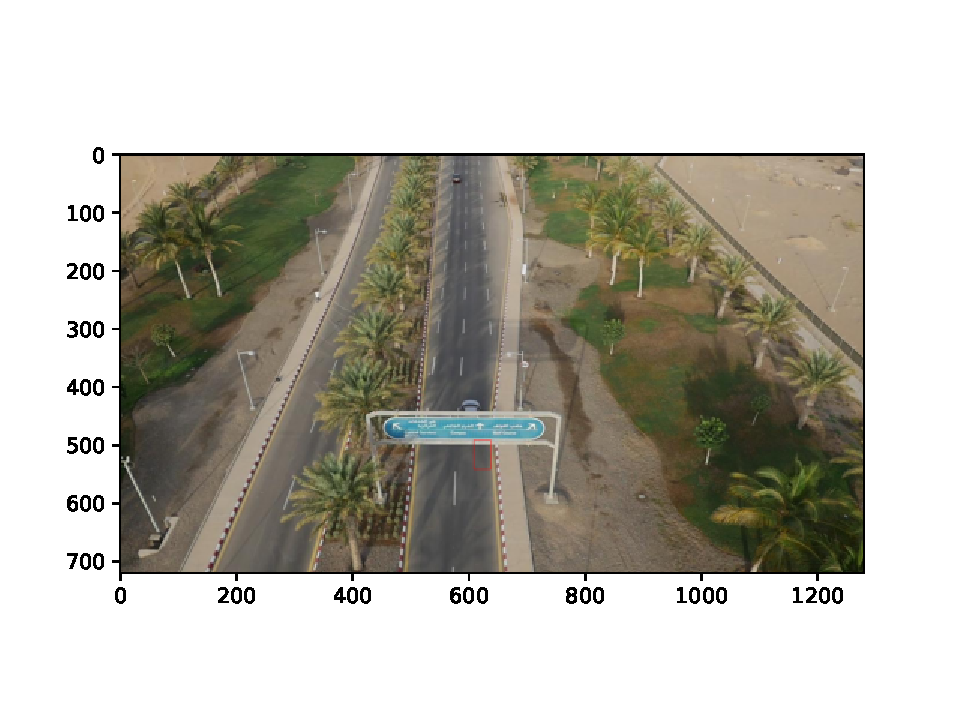
\includegraphics[width=\textwidth]{st_example.pdf}
        \caption{Short-term tracker looses target after occlusion.}
    \end{subfigure}
    \begin{subfigure}{0.522\textwidth}
        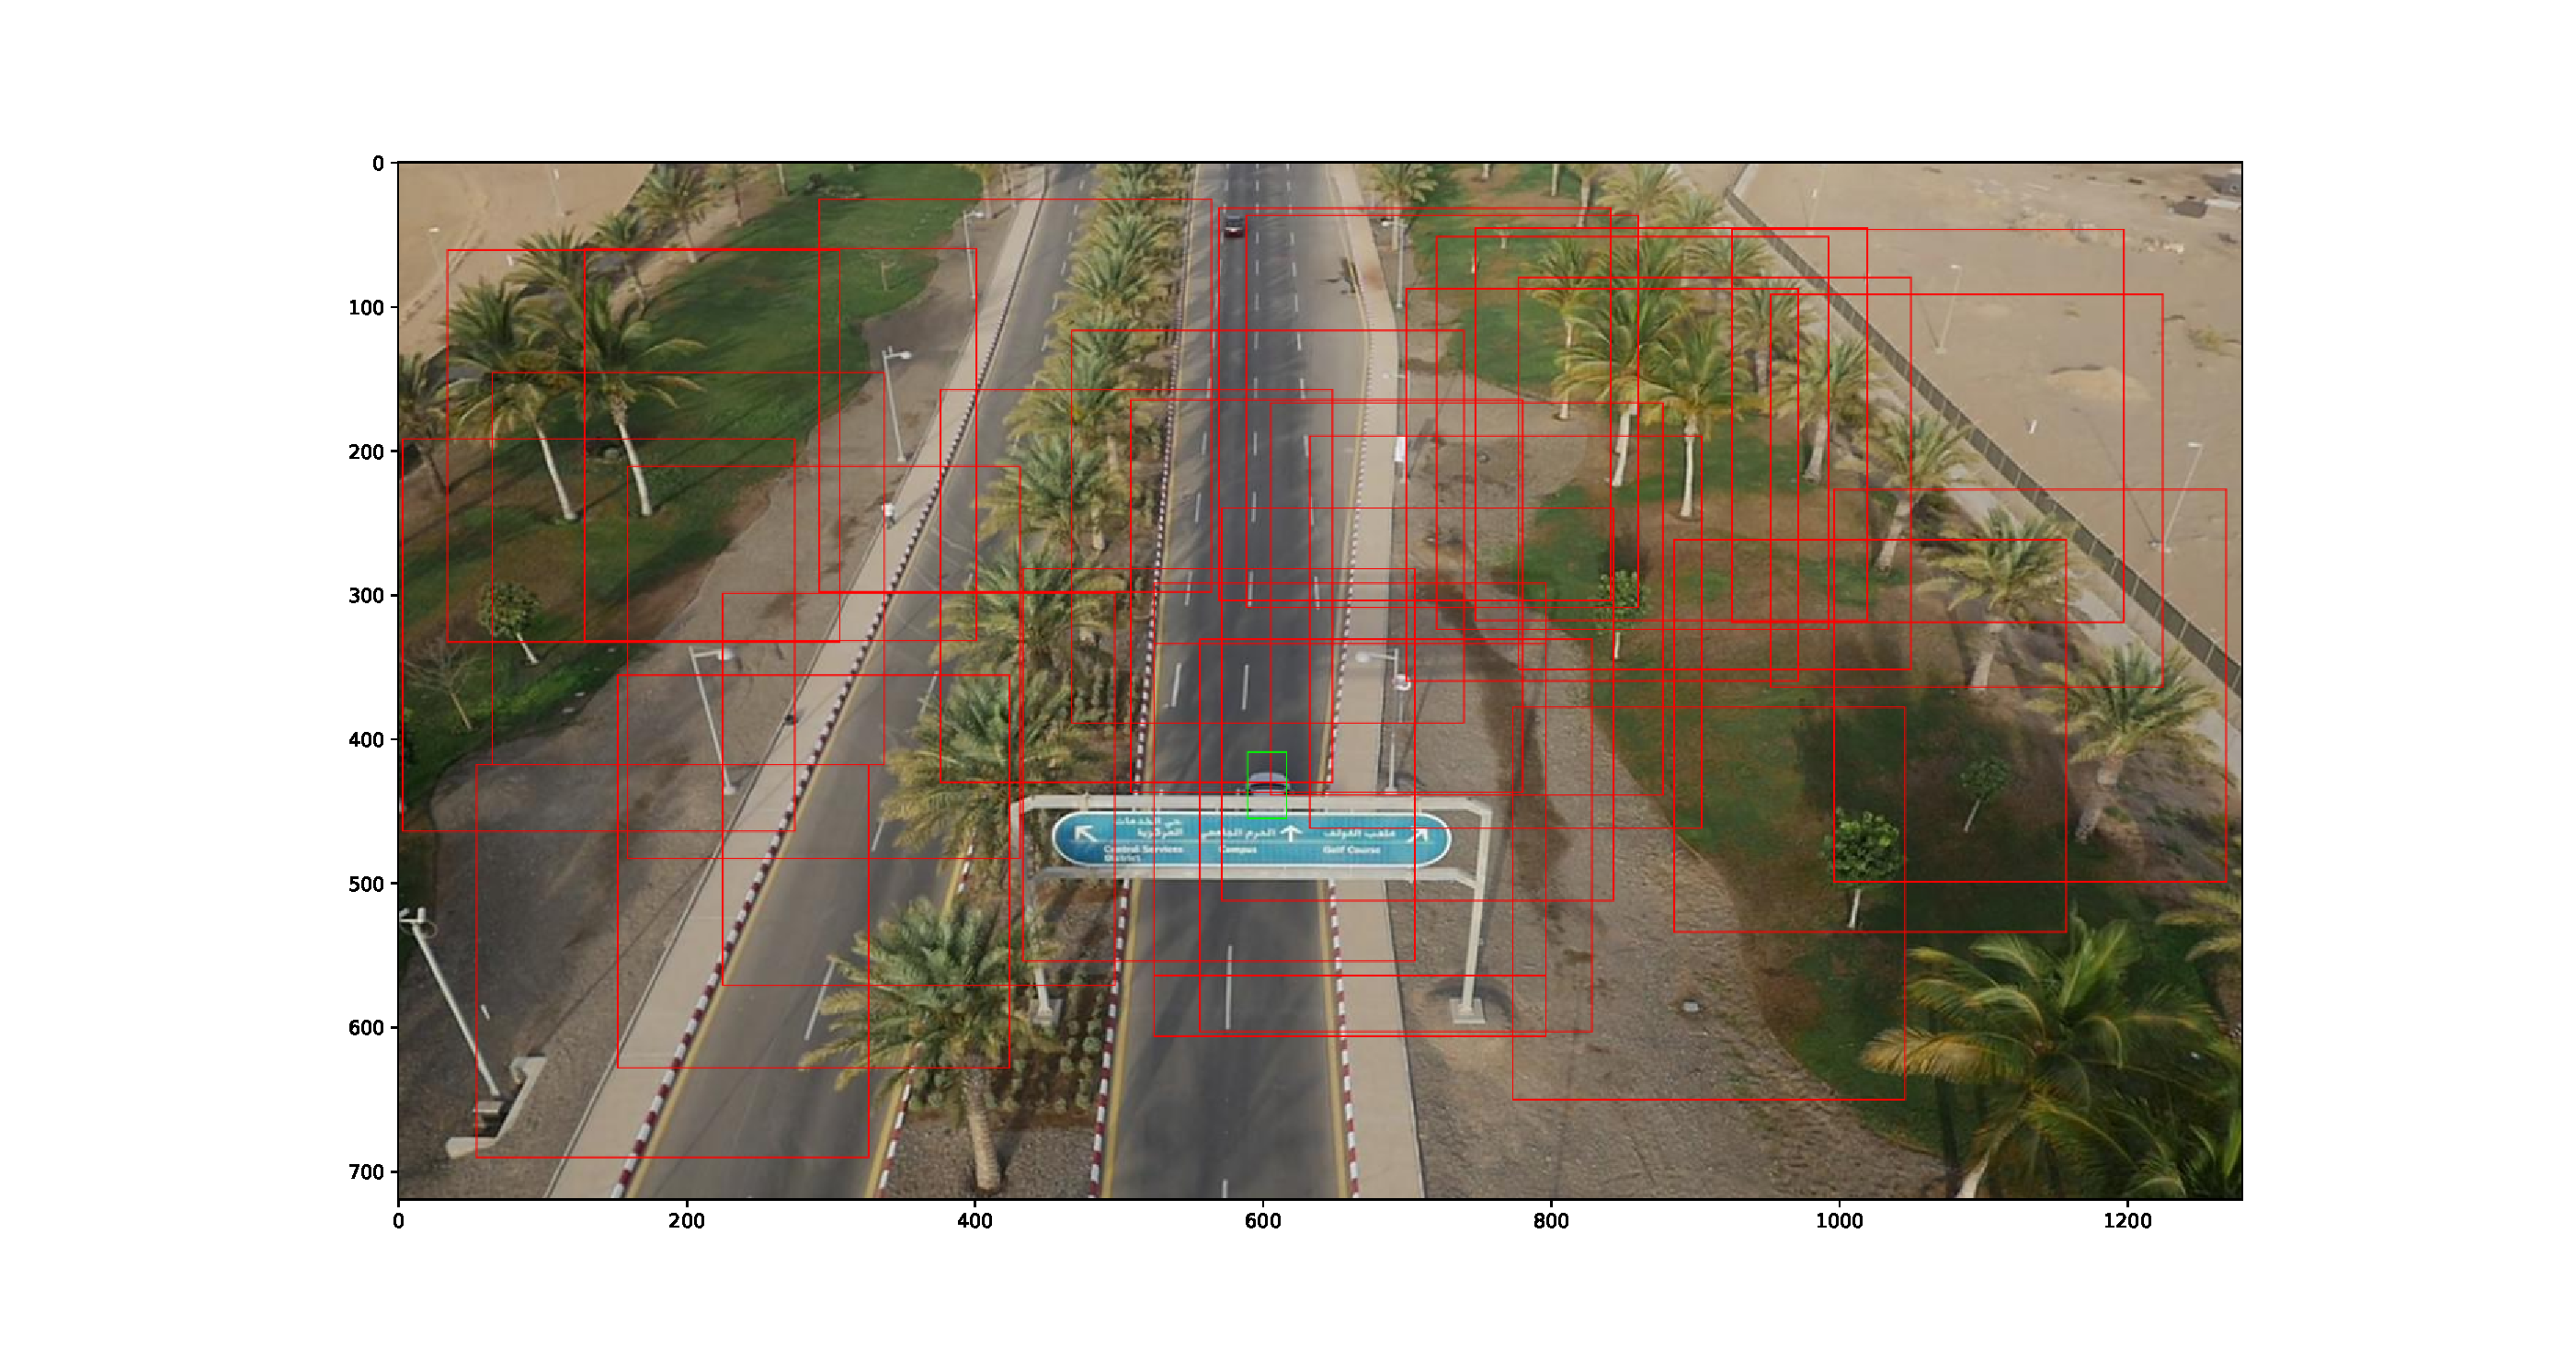
\includegraphics[width=\textwidth]{longterm_ecxample.pdf}
        \caption{Long-term tracker and the new samples of possible locations in red.}
    \end{subfigure}
    \caption{Example of short-term and long-term tracking.}
    \label{fig:tracking}
\end{figure}




\section{Conclusion}
Even a simple re-detection procedure can increase the tracking performance.
Using adtional stratagies like video stabilization using Lucas-kanade and Kalman filtering could further improve the tracking performance.
The drawback of this implementation is the number of samples that has to be drawn, leading to a drop in FPS performance.


\bibliographystyle{IEEEtran}
\bibliography{bibliography}

\end{document}
